% vim: set textwidth=120:

% Example CV based on the 1.5-column-cv template. Main features:
% * uses the Roboto font family and IcoMoon icon set;
% * doesn't use colours, different font weights are used instead for styling;
% * because the CV fits on one page, header and footer is empty, since there isn't much useful info to put there;
% * includes a photo.
\documentclass[a4paper,10pt]{article}


% package imports
% ---------------

\usepackage[british]{babel} % for correct language and hyphenation and stuff
\usepackage{calc}           % for easier length calculations (infix notation)
\usepackage{enumitem}       % for configuring list environments
\usepackage{fancyhdr}       % for setting header and footer
\usepackage{fontspec}       % for fonts
\usepackage{geometry}       % for setting margins (\newgeometry)
\usepackage{graphicx}       % for pictures
\usepackage{microtype}      % for microtypography stuff
\usepackage{xcolor}         % for colours
\usepackage{datetime}
\usepackage{hyperref}
\usepackage{shadowtext}



% margin and column widths
% ------------------------

% margins
\newgeometry{left=8mm,right=15mm,top=15mm,bottom=15mm}

% width of the gap between left and right column
\newlength{\cvcolumngapwidth}
\setlength{\cvcolumngapwidth}{3.5mm}

% left column width
\newlength{\cvleftcolumnwidth}
\setlength{\cvleftcolumnwidth}{42.5mm}

% right column width
\newlength{\cvrightcolumnwidth}
\setlength{\cvrightcolumnwidth}{\textwidth-\cvleftcolumnwidth-\cvcolumngapwidth}

% set paragraph indentation to 0, because it screws up the whole layout otherwise
\setlength{\parindent}{0mm}


% style definitions
% -----------------
% style categories explanation:
% * \cvnameXXX is used for the name;
% * \cvsectionXXX is used for section names (left column, accompanied by a horizontal rule);
% * \cvtitleXXX is used for job/education titles (right column);
% * \cvdurationXXX is used for job/education durations (left column);
% * \cvheadingXXX is used for headings (left column);
% * \cvmainXXX (and \setmainfont) is used for main text;
% * \cvruleXXX is used for the horizontal rules denoting sections.

% font families
\defaultfontfeatures{Ligatures=TeX} % reportedly a good idea, see https://tex.stackexchange.com/a/37251

% Configure a directory location for fonts(default: 'fonts/')
\newcommand*{\fontdir}[1][fonts/]{\def\@fontdir{#1}}
\fontdir


\newfontfamily{\cvnamefont}{Roboto Medium}
\newfontfamily{\cvsectionfont}{Roboto Medium}
\newfontfamily{\cvtitlefont}{Roboto Regular}
\newfontfamily{\cvdurationfont}{Roboto Light Italic}
\newfontfamily{\cvheadingfont}{Roboto Regular}
\newfontfamily{\cvhonorfont}{Roboto Medium}
\newfontfamily{\cvboldfont}[Path=\@fontdir,Scale=1]{OpenSans-SemiBold}
\newfontfamily{\cvskillfont}[Path=\@fontdir,Scale=1]{OpenSans-SemiBoldItalic}
\setmainfont{Roboto Light}

% colours
\definecolor{cvnamecolor}{HTML}{000000}
\definecolor{cvsectioncolor}{HTML}{3366ff}
\definecolor{cvtitlecolor}{HTML}{000000}
\definecolor{cvdurationcolor}{HTML}{000000}
\definecolor{cvheadingcolor}{HTML}{000000}
\definecolor{cvmaincolor}{HTML}{000000}
\definecolor{cvrulecolor}{HTML}{000000}
\definecolor{cvwhatcolor}{HTML}{5588ff}
\definecolor{cvwherecolor}{HTML}{656565}
\definecolor{cvnoskillcolor}{HTML}{d9d9d9}
\definecolor{cvboldcolor}{HTML}{808080}
\definecolor{cvskilledcolor}{HTML}{668cff}
\color{cvmaincolor}

% styles
\newcommand{\cvnamestyle}[1]{{\Large\cvnamefont\textcolor{cvnamecolor}{#1}}}
\newcommand{\cvsectionstyle}[1]{{\normalsize\cvsectionfont\textcolor{cvsectioncolor}{#1}}}
\newcommand{\cvtitlestyle}[1]{{\large\cvtitlefont\textcolor{cvtitlecolor}{#1}}}
\newcommand{\cvdurationstyle}[1]{{\small\cvdurationfont\textcolor{cvdurationcolor}{#1}}}
\newcommand{\cvheadingstyle}[1]{{\normalsize\cvheadingfont\textcolor{cvheadingcolor}{#1}}}
\newcommand{\cvboldstlye}[1]{{\normalsize\cvboldfont\textcolor{cvboldcolor}{\scalebox{.93}[1.0]{#1}}}}
\newcommand{\cvskillstlye}[1]{{\normalsize\cvskillfont\textcolor{cvwherecolor}{\scalebox{.95}[1.0]{#1}}}}

% Date time format
\newdateformat{monthyeardate}{%
  \THEDAY \space \monthname[\THEMONTH] \THEYEAR}


% inter-item spacing
% ------------------

% vertical space after personal info and standard CV items
\newlength{\cvafteritemskipamount}
\setlength{\cvafteritemskipamount}{5mm plus 1.25mm minus 1.25mm}

% vertical space after other items
\newlength{\cvafterotheritemskipamount}
\setlength{\cvafterotheritemskipamount}{2mm plus 1mm minus 1mm}


% vertical space after sections
\newlength{\cvaftersectionskipamount}
\setlength{\cvaftersectionskipamount}{1mm plus 0.5mm minus 0.5mm}

% extra vertical space to be used when a section starts with an item with a heading (e.g. in the skills section),
% so that the heading does not follow the section name too closely
\newlength{\cvbetweensectionandheadingextraskipamount}
\setlength{\cvbetweensectionandheadingextraskipamount}{1mm plus 0.25mm minus 0.25mm}


% intra-item spacing
% ------------------

% vertical space after name
\newlength{\cvafternameskipamount}
\setlength{\cvafternameskipamount}{3mm plus 0.75mm minus 0.75mm}

% vertical space after personal info lines
\newlength{\cvafterpersonalinfolineskipamount}
\setlength{\cvafterpersonalinfolineskipamount}{2mm plus 0.5mm minus 0.5mm}

% vertical space after titles
\newlength{\cvaftertitleskipamount}
\setlength{\cvaftertitleskipamount}{1mm plus 0.25mm minus 0.25mm}

% value to be used as parskip in right column of CV items and itemsep in lists (same for both, for consistency)
\newlength{\cvparskip}
\setlength{\cvparskip}{0.5mm plus 0.125mm minus 0.125mm}

% set global list configuration (use parskip as itemsep, and no separation otherwise)
\setlist{parsep=0mm,topsep=0mm,partopsep=0mm,itemsep=\cvparskip}


% CV commands
% -----------

% creates a "personal info" CV item with the given left and right column contents, with appropriate vertical space after
% @param #1 left column content (should be the CV photo)
% @param #2 right column content (should be the name and personal info)
\newcommand{\cvpersonalinfo}[2]{
    % left and right column
    \begin{minipage}[t]{\cvleftcolumnwidth}
        \vspace{0mm} % XXX hack to align to top, see https://tex.stackexchange.com/a/11632
        \raggedleft #1
    \end{minipage}% XXX necessary comment to avoid unwanted space
    \hspace{\cvcolumngapwidth}% XXX necessary comment to avoid unwanted space
    \begin{minipage}[t]{\cvrightcolumnwidth}
        \vspace{0mm} % XXX hack to align to top, see https://tex.stackexchange.com/a/11632
        #2
    \end{minipage}

    % space after
    \vspace{\cvafteritemskipamount}
}

% typesets a name, with appropriate vertical space after
% @param #1 name text
\newcommand{\cvname}[1]{
    % name
    \cvnamestyle{#1}

    % space after
    \vspace{\cvafternameskipamount}
}

% typesets a line of personal info beginning with an icon, with appropriate vertical space after
% @param #1 parameters for the \includegraphics command used to include the icon
% @param #2 icon filename
% @param #3 line text
\newcommand{\cvpersonalinfolinewithicon}[3]{
    % icon, vertically aligned with text (see https://tex.stackexchange.com/a/129463)
    \raisebox{.5\fontcharht\font`E-.5\height}{\includegraphics[#1]{#2}}
    % text
    #3

    % space after
    \vspace{\cvafterpersonalinfolineskipamount}
}

% creates a "section" CV item with the given left column content, a horizontal rule in the right column, and with
% appropriate vertical space after
% @param #1 left column content (should be the section name)
\newcommand{\cvsection}[1]{
    % left and right column
    \begin{minipage}[t]{\cvleftcolumnwidth}
        \raggedleft\cvsectionstyle{#1}
    \end{minipage}% XXX necessary comment to avoid unwanted space
    \hspace{\cvcolumngapwidth}% XXX necessary comment to avoid unwanted space
    \begin{minipage}[t]{\cvrightcolumnwidth}
        \textcolor{cvrulecolor}{\rule{\cvrightcolumnwidth}{0.3mm}}
    \end{minipage}

    % space after
    \vspace{\cvaftersectionskipamount}
}

% creates a standard, multi-purpose CV item with the given left and right column contents, parskip set to cvparskip
% in the right column, and with appropriate vertical space after
% @param #1 left column content
% @param #2 right column content
\newcommand{\cvitem}[2]{
    % left and right column
    \begin{minipage}[t]{\cvleftcolumnwidth}
        \raggedleft #1
    \end{minipage}% XXX necessary comment to avoid unwanted space
    \hspace{\cvcolumngapwidth}% XXX necessary comment to avoid unwanted space
    \begin{minipage}[t]{\cvrightcolumnwidth}
        \setlength{\parskip}{\cvparskip} #2
    \end{minipage}

    % space after
    \vspace{\cvafteritemskipamount}
}

\newcommand{\cvhonoritem}[2]{
    % left and right column
    \begin{minipage}[t]{\cvleftcolumnwidth}
        \raggedleft #1
    \end{minipage}% XXX necessary comment to avoid unwanted space
    \hspace{\cvcolumngapwidth}% XXX necessary comment to avoid unwanted space
    \begin{minipage}[t]{\cvrightcolumnwidth}
        \setlength{\parskip}{\cvparskip} #2
    \end{minipage}

    % space after
    \vspace{1.7mm}
}


\newcommand{\cvotheritem}[2]{
    % left and right column
    \begin{minipage}[t]{\cvleftcolumnwidth}
        \raggedleft #1
    \end{minipage}% XXX necessary comment to avoid unwanted space
    \hspace{\cvcolumngapwidth}% XXX necessary comment to avoid unwanted space
    \begin{minipage}[t]{\cvrightcolumnwidth}
        \setlength{\parskip}{\cvparskip} #2
    \end{minipage}

    % space after
    \vspace{\cvafterotheritemskipamount}
}
% typesets a title, with appropriate vertical space after
% @param #1 title text
\newcommand{\cvtitle}[1]{
    % title
    \cvtitlestyle{#1}

    % space after
    \vspace{\cvaftertitleskipamount}
    % XXX need to subtract cvparskip here, because it is automatically inserted after the title "paragraph"
    \vspace{-\cvparskip}
}

% cv Skill Bar
\makeatletter
\newdimen\skillb@level
\newdimen\skillb@length
\newdimen\skillb@height
\skillb@length=89pt%
\skillb@height=8pt%
\newcommand*{\skillbar}[1]{%
    \skillb@level=\dimexpr#1\skillb@length/100\relax%
    {\color{cvskilledcolor}\rule{\skillb@level}{\skillb@height}}%
    {\color{cvnoskillcolor}%
        \rule{\dimexpr\skillb@length-\skillb@level\relax}{\skillb@height}}%

}
\makeatother

% header and footer
% -----------------

% set empty header and footer
\pagestyle{empty}



% preamble end/document start
% ===========================

\begin{document}



% personal info
% -------------

\cvpersonalinfo{
    % photo
    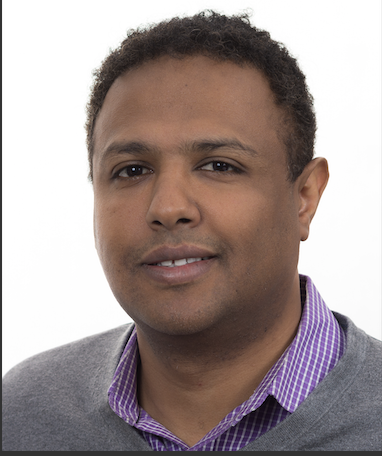
\includegraphics[height=36.5mm]{samprofile.png}
    }{
    % name
    \cvname{Samuel Haile}

    % address
    \cvpersonalinfolinewithicon{height=4mm}{072-location.pdf}{
        New Castle, DE, 19720
    }

    % phone number
    \cvpersonalinfolinewithicon{height=4mm}{067-phone.pdf}{
        +1 267-934-0203
    }

    % email address
    \cvpersonalinfolinewithicon{height=4mm}{070-envelop.pdf}{
        \href{mailto:samishken@gmail.com}{samishken@gmail.com}
    }

    % LinkedIn account
    \cvpersonalinfolinewithicon{height=4mm}{458-linkedin.pdf}{
        \href{https://www.linkedin.com/in/samuel-haile-ga/}{samuel-haile}
    }




}

% skills
% ------

\cvsection{\textbf{SKILLS}}

\vspace{\cvbetweensectionandheadingextraskipamount}


%  skills
\cvitem{
    \cvheadingstyle{Engineering Software}

}{
        \setlength\tabcolsep{5pt}
        \begin{tabular}{|l|l|l|l|}

        Python   & R   & C/C++  & Bash \\
        \footnotesize{\emph{H2o API, AWS boto, airflow }} &
        \footnotesize{\emph{RStudio, SparklyR, H2o}} &
        \footnotesize{\emph{RMPI, CUDA, CMetrics }} &
        \footnotesize{\emph{RHEL/Ubuntu, RPMs}}\\

        \footnotesize{\emph{Tensor Flow, Keras}} &
         \footnotesize{\emph{REST API, CRAN}} &
         \footnotesize{\emph{gcc, cmake}} &
         \footnotesize{\emph{git, HDFS, Apache }}\\


        \end{tabular}
}

% completely vetted skills
\vspace{-2mm}
\cvitem{
    \cvheadingstyle{Programming Languages}

}{
        \setlength\tabcolsep{5pt}
        \begin{tabular}{|l|l|l|l|}
        SQL  & AWS API & Javascript & Java \\
         \footnotesize{\emph{DynamoDB, RedShift}} &
         \footnotesize{\emph{ELK stack, S3}} &
         \footnotesize{\emph{Chrome DevTools, Flow}} &
         \footnotesize{\emph{Hadoop, oozie, Scala }}\\

         \footnotesize{\emph{Code Deploy, Code Commit }} &
         \footnotesize{\emph{Docker, Amazon EMR }} &
         \footnotesize{\emph{Yarn, Postmates}} &
         \footnotesize{\emph{RapidMiner}}\\



        \end{tabular}
 }





% work experience
% ---------------

\cvsection{\textbf{WORK EXPERIENCE}}

% Company 1 current
\cvitem{
    \cvdurationstyle{August 2017 -- present}
}{
    \cvtitle{DATA SCIENCE MANAGER - AI Framework Development \& Testing}

    \textcolor{cvwhatcolor}{\emph{\textbf{DATA SCIENCE MANAGER}}}
    \textcolor{cvwherecolor}{\textbf{\textbar}}
    \textcolor{cvwherecolor}{\emph{\textbf{LOTUS-X GROUP - Philadelphia, PA}}}

    \begin{itemize}[leftmargin=*]
        \item Developed a variety of Machine Learning Pipelines and managed various stages of the delivery process including post-service stages.
        \item Performed detailed feature engineering, code logging and automated data-leakage testing.
        \item Set up automated parallel Data Pipelines for various projects with Amazon SageMaker, AWS Workflow and several other services.
        \item Delivered {\cvboldstlye{PhillyTalent, Recommendation System API} 07.2018 - 10.2018}
        \item Delivered {\cvboldstlye{Anaheim, Predictive Demand Model for Gas Stations} 10.2018 - present}
        \item Delivered {\cvboldstlye{Welder Classifier, AI-Enabled performance Evaluator, Airgas} 03.2018 - 05.2018}
        \item Delivered {\cvboldstlye{XPhilly, Automated E-Commerce Data ETL} 07.2018 - 10.2018}
        \item Presented {\cvboldstlye{Workshop: State of the Art Streaming Learning with Vowpal Wabbit} 08.2018}
        \item Delivered {\cvboldstlye{PhillyTalent, Recommendation System API} 07.2018 - 10.2018}

    \end{itemize}
}


%  Company 3
\cvitem{
    \cvdurationstyle{June 2015 -- August 2017}
}{
    \cvtitle{FOUNDER}

   \textcolor{cvwhatcolor}{\emph{\textbf{{FOUNDER}}}}
    \textcolor{cvwherecolor}{\textbf{\textbar}}
    \textcolor{cvwherecolor}{\emph{\textbf{LOTUS INDUSTRIES AND CONSULTING GROUP - State College, PA}}}

\begin{itemize}[leftmargin=*]
       \item Conducted testing on the legacy IBM GPFS module, both on Batch and Interactive systems, for R, Python and several other commercial and opensource computing packages.
       \item Developed new training R Packages for ParallelR and RHadoop for faculty clients.

   \end{itemize}



}


%  Company 3
\cvitem{
    \cvdurationstyle{January 2013 -- March 2013}
}{
    \cvtitle{PROJECT MANAGER SCHOLAR}

   \textcolor{cvwhatcolor}{\emph{\textbf{{PROJECT MANAGER SCHOLAR}}}}
    \textcolor{cvwherecolor}{\textbf{\textbar}}
    \textcolor{cvwherecolor}{\emph{\textbf{GOOGLE - San Francisco, CA}}}


Led my team to develop a Payment Android App in collaboration with the Google Wallet team, using NFC sensor Technology and Google Wallet APIs for secure transactions and ran a demo to a panel of C-level managers.

}
% Company 2
\cvitem{
    \cvdurationstyle{September 2011 -- June 2015}
}{
    \cvtitle{APPLICATION SPECIALIST}

    \textcolor{cvwhatcolor}{\emph{\textbf{APPLICATION SPECIALIST}}}
    \textcolor{cvwherecolor}{\textbf{\textbar}}
    \textcolor{cvwherecolor}{\emph{\textbf{PENN STATE INSTITUTE OF CYBERSCIENCE - State College, PA}}}

 \begin{itemize}[leftmargin=*]
       \item   Delivered Statistics Application support and Parallel Computing solutions on a variety of topics and technical levels over the years to the research and industry partners of Penn State computing clusters resources.
       \item Managed commercial licenses, package versioning and deployment across all clusters
       \item Performed user account maintenance and access-policy tests and updates.


   \end{itemize}
}



}

%  Company 3
\cvitem{
    \cvdurationstyle{January 2011 -- September 2011}
}{
    \cvtitle{RESEARCH ASSISTANT}

   \textcolor{cvwhatcolor}{\emph{\textbf{{RESEARCH ASSISTANT}}}}
    \textcolor{cvwherecolor}{\textbf{\textbar}}
    \textcolor{cvwherecolor}{\emph{\textbf{PENN STATE - State College, PA}}}

\begin{itemize}[leftmargin=*]
       \item Prototyped different algorithms for Big(O) evaluation, profiling and complexity analysis.


   \end{itemize}
}

\vspace{3mm}
\pagebreak
% education
% ---------

\cvsection{\textbf{EDUCATION}}



% master's
\cvitem{
    \cvdurationstyle{August 2009 -- December 2012}
}{
    \cvtitle{Masters of Engineering in Aerospace Engineering}

     \textcolor{cvwhatcolor}{\emph{\textbf{Master of Engineering}}}
    \textcolor{cvwherecolor}{\textbf{\textbar}}
    \textcolor{cvwherecolor}{\emph{\textbf{Aerospace Eng}}}
     \textcolor{cvwherecolor}{\textbf{\textbar}}
     \textcolor{cvwherecolor}{\emph{\textbf{Pennsylvania State University-Main Campus, State College, PA}}}

    \begin{itemize}[leftmargin=*]
        \item Paper: \emph{Risk Visualization and Uncertainty Quantification}


    \end{itemize}
}
% certificate program
\cvitem{
    \cvdurationstyle{January 2010 -- September 2012 \\ 21/30 Cred}
}{
    \cvtitle{Certificate Applied Statisitcs}

    \textcolor{cvwhatcolor}{\emph{\textbf{Graduate Certificate}}}
    \textcolor{cvwherecolor}{\textbf{\textbar}}
    \textcolor{cvwherecolor}{\emph{\textbf{Applied Statistics}}}
     \textcolor{cvwherecolor}{\textbf{\textbar}}
     \textcolor{cvwherecolor}{\emph{\textbf{Pennsylvania State University-Main Campus, State College, PA}}}

    \begin{itemize}[leftmargin=*]
        \item Subjects: Partial Differential Equations | Neural Networks Control | Estimation Theory

    \end{itemize}
}


% Projects Undertaken
%-------

\cvsection{\textbf{SUMMARY OF PRIOR PUBLICATIONS, AWARDS & PROJECTS}}

\vspace{\cvbetweensectionandheadingextraskipamount}

% project 1
\cvitem{
    \cvdurationstyle{2011 -- 2017}
    }
{
    \cvtitle{Additional Information}
    \textcolor{cvwhatcolor}{\emph{\textbf{{Penn State}}}}
    \textcolor{cvwherecolor}{\textbf{\textbar}}
    \textcolor{cvwherecolor}{\emph{\textbf{Pennsylvania State University-Main Campus, State College, PA}}}

\begin{itemize}[leftmargin=*]
        \item 2017 Top 4/32 , AirLiquide, B2B Machine Learning Chapter, Philadelphia
        \item 2013 Finalist , Princeton Competition, for BeautifulWave

        \item  2013 National, top 120 University Olympics, San Francisco, CA

        \item 2013 1st/63 , University Olympics, Penn State
        \item 2012 2nd, Penn StatSe, for inDistance Android mobile App
        \item 2012 Full Scholarship, Information Science and Technology Dept. , Penn State
        \item 2011 3+ CITATIONS, Optimum Vibration Design of Fiber Metal Laminated Panels by Particle Swarm Optimization Algorithm
        \item 2011 3+ CITATIONS , Free Vibration Analysis of Rotating Laminated Composite Panels Using Finite Strip Method
        \item 2011 Full Scholarship, Information Technology Services, Penn State

    \end{itemize}

}
% project 2
\cvitem{
    \cvdurationstyle{ 2009 --  2010}
    }
{
    \cvtitle{MIT OpenCourseWare:}
        \textcolor{cvwhatcolor}{\emph{\textbf{{MIT OpenCourseWare:}}}}


    \begin{itemize}[leftmargin=*]

        \item Pattern Matching and Rule-based Substitution.  \href{https://www.youtube.com/watch?v=amf5lTZ0UTc}{Published Link}
        \item Storage Allocation and Garbage Collection. \href{https://www.youtube.com/watch?v=2s2_FAf-yQs}{Published Link}
        \item Structure and Interpretation of Computer Programs.  \href{https://www.youtube.com/watch?v=2Op3QLzMgSY}{Published Link}

    \end{itemize}
}

% project 3
\cvitem{
    \cvdurationstyle{ 2012 --  2013}
    }
{
    \cvtitle{Papers}
        \textcolor{cvwhatcolor}{\emph{\textbf{{ Papers:}}}}


    \begin{itemize}[leftmargin=*]

    \item H Pourzand, MH Sadr, Optimum Vibration Design of Fiber Metal Laminated Panels by Particle Swarm Optimization Algorithm, International Mechanical Engineering Congress and Exposition, 805-811, ASME 2011. \href{http://proceedings.asmedigitalcollection.asme.org/proceeding.aspx?articleid=1644927}{Published Link}


    \end{itemize}
}

%\cvsection{\textbf{ACCOLADES}}
%
%\vspace{\cvbetweensectionandheadingextraskipamount}
%
%% Award 1
%\cvhonoritem{
%    \cvdurationstyle{November 2018}
%    }
%{
%     \cvtitlestyle{Winner - TECHiQ Contest} \textcolor{cvwherecolor}{\textbf{\textbar}} \emph{for the most technologically sound 6-member team among 1400+ employees across all L\&T Defence locations} \cvdurationstyle{@}
%   \textcolor{cvwhatcolor}{\emph{\textbf{{Larsen \& Toubro Limited, Mumbai}}}}
%}




% additional info
% ---------------

\cvsection{\textbf{ADDITIONAL DETAILS}}

\vspace{\cvbetweensectionandheadingextraskipamount}

% interests
\cvotheritem{
   \cvheadingstyle{Summmary \& Details}
}{
    \emph{   }
    {
  \cvtitle{MIT OpenCourseWare:}
      \textcolor{cvwhatcolor}{\emph{\textbf{{Code Repositories }}}}
    \begin{itemize}[leftmargin=*]

        \item LAN Meetup: Leverage AWS Now Workshops 2017 - present,
        \href{https://www.meetup.com/Leverage-AWS-Now-Philadelphia}{Published Link}
        \item GitHub Repo 2017 - present,
        \href{https://github.com/lotusxai}{Published Link}
        \item GitHub Repo 2012 - 2016,
        \href{https://github.com/office206}{Published Link}
        \item GitHub Repo 2009 - 2012,
        \href{https://github.com/hup128}{Published Link}

    \end{itemize}
}
}


% skills
% ------

\cvsection{\textbf{DevOps}}

\vspace{\cvbetweensectionandheadingextraskipamount}


%  skills
\cvitem{
    \cvheadingstyle{Engineering Software}

}{
        \setlength\tabcolsep{5pt}
        \begin{tabular}{|l|l|l|l|}

        Analytics   & DevOps   & DevOps/Other  & DevOps/Other \\
        \footnotesize{\emph{Apache Superset }} &
        \footnotesize{\emph{Docker, Docker Compose }} &
        \footnotesize{\emph{Travis CI, Locust, CloudWatch }} &
        \footnotesize{\emph{codecov.io, Vault, Slack}}\\

        \footnotesize{\emph{Databricks }} &
         \footnotesize{\emph{Packer, localstack, readthedocs}} &
         \footnotesize{\emph{Talend Data Stream, cloudcraft}} &
         \footnotesize{\emph{Jira, Sphinx-docs, \LaTeX  }}\\


        \end{tabular}
}


\vspace{3mm}





%cvsection{\textbf{}}

\vspace{0.3cm}


\end{document}